\documentclass[aspectratio=169]{beamer}
% Shared preamble for ml/ slide decks.
% Each lecture .tex starts with:
%   \documentclass[aspectratio=169]{beamer}
%   % Shared preamble for ml/ slide decks.
% Each lecture .tex starts with:
%   \documentclass[aspectratio=169]{beamer}
%   % Shared preamble for ml/ slide decks.
% Each lecture .tex starts with:
%   \documentclass[aspectratio=169]{beamer}
%   \input{../preamble}
% Compile from inside the chapter folder so \input{../preamble} resolves.

\usetheme{default}
\usecolortheme{dove}

\setbeamertemplate{navigation symbols}{}
\setbeamertemplate{footline}{%
  \hfill{\large\insertframenumber\,/\,\inserttotalframenumber}\hspace{0.8em}\vspace{0.5em}%
}

% Project palette (existing, kept for backwards compatibility with deferred/*)
\definecolor{popblue}{RGB}{52, 101, 164}
\definecolor{sampred}{RGB}{204, 0, 0}
\definecolor{paramgreen}{RGB}{0, 140, 70}
\definecolor{warnred}{RGB}{180, 40, 40}
\definecolor{orange1}{RGB}{220, 120, 0}
\definecolor{violet1}{RGB}{120, 50, 160}
\definecolor{lightbg}{RGB}{245, 245, 250}

% Armenian flag palette (use these for any 3-color highlight; per CLAUDE.md).
% "Nice versions": slightly de-saturated from the official spec for slide use,
% so they don't burn out under projector colors. Originals kept as *_pure.
\definecolor{armred}{RGB}{200, 30, 40}      % nice red (official #D90012 muted)
\definecolor{armblue}{RGB}{30, 70, 160}     % nice blue (official #0033A0 muted)
\definecolor{armorange}{RGB}{230, 160, 30}  % nice orange (official #F2A800 muted)
\definecolor{armred_pure}{HTML}{D90012}     % official Armenian flag red
\definecolor{armblue_pure}{HTML}{0033A0}    % official Armenian flag blue
\definecolor{armorange_pure}{HTML}{F2A800}  % official Armenian flag orange

\setbeamercolor{frametitle}{fg=popblue}
\setbeamercolor{title}{fg=popblue}

\usepackage{pgfplots}
\usepackage{tikz}
\usetikzlibrary{shapes, arrows.meta, positioning, calc, decorations.pathreplacing, patterns, matrix}
\pgfplotsset{compat=1.18}
\usepackage{amsmath, amssymb, amsfonts}
\usepackage{bm}
\usepackage{dsfont}
\usepackage{array}
\usepackage{pifont}
\usepackage{colortbl}
\usepackage{fontenc}

% Callout boxes. Purely additive - existing decks are unaffected.
% Usage: \begin{tcolorbox}[colback=armblue!8, colframe=armblue, boxrule=0.6pt, arc=2pt,
%                          title=\textbf{Key idea}] ... \end{tcolorbox}
% Palette convention (ml/SLIDE_STYLE.md): armblue=key idea, armred=trap/warning,
% paramgreen=takeaway or "Next", armorange=watch-out.
\usepackage[most]{tcolorbox}

% Cleaner table rules (\toprule, \midrule, \bottomrule). Also purely additive.
\usepackage{booktabs}

% \cancel{...} for struck-through terms in derivations (added 2026-08-11 for the
% importance-sampling frame in ch11_rl, where the dynamics cancel). Purely additive.
\usepackage{cancel}

% Minimal ML notation macros (subset of slds-lmu latex-math/basic-ml.tex).
% Kept here so we don't have to inline-expand every \thetav, \xv, etc.
% when porting upstream slides.
\newcommand{\R}{\mathds{R}}
\newcommand{\N}{\mathds{N}}
\newcommand{\E}{\mathds{E}}
\newcommand{\Xspace}{\mathcal{X}}
\newcommand{\Yspace}{\mathcal{Y}}
\newcommand{\Hspace}{\mathcal{H}}
\newcommand{\D}{\mathcal{D}}
\newcommand{\Dtrain}{\mathcal{D}_{\text{train}}}
\newcommand{\Dtest}{\mathcal{D}_{\text{test}}}
\newcommand{\xv}{\mathbf{x}}
\newcommand{\yv}{\mathbf{y}}
\newcommand{\Xmat}{\mathbf{X}}
\newcommand{\id}{\mathbf{I}}
\newcommand{\thetav}{\bm{\theta}}
\newcommand{\thetah}{\hat{\bm{\theta}}}
\newcommand{\lamv}{\bm{\lambda}}
\newcommand{\fx}{f(\xv)}
\newcommand{\fxt}{f(\xv \,|\, \bm{\theta})}
\newcommand{\fxi}{f\!\left(\xv^{(i)}\right)}
\newcommand{\fh}{\hat{f}}
\newcommand{\fxh}{\hat{f}(\xv)}
\newcommand{\yh}{\hat{y}}
\newcommand{\yih}{\hat{y}^{(i)}}
% \xi clashes with the Greek letter \xi; write \xv^{(i)} inline instead.
\newcommand{\yi}[1][i]{y^{(#1)}}
\newcommand{\xyi}[1][i]{\left(\xv^{(#1)},\, y^{(#1)}\right)}
\newcommand{\thx}{\bm{\theta}^\top \xv}
\newcommand{\sumin}{\sum_{i=1}^{n}}
\newcommand{\sumjp}{\sum_{j=1}^{p}}
\newcommand{\Lxy}{L\!\left(y, \fx\right)}
\newcommand{\Lxyi}{L\!\left(\yi, \fxi\right)}
\newcommand{\risk}{\mathcal{R}}
\newcommand{\riske}{\mathcal{R}_{\text{emp}}}
\newcommand{\risket}{\mathcal{R}_{\text{emp}}(\bm{\theta})}
\newcommand{\riskt}{\mathcal{R}(\bm{\theta})}
\newcommand{\riskr}{\mathcal{R}_{\text{reg}}}
\newcommand{\argmin}{\mathop{\mathrm{arg\,min}}}
\newcommand{\argmax}{\mathop{\mathrm{arg\,max}}}
\newcommand{\eps}{\varepsilon}

% Compile from inside the chapter folder so % Shared preamble for ml/ slide decks.
% Each lecture .tex starts with:
%   \documentclass[aspectratio=169]{beamer}
%   \input{../preamble}
% Compile from inside the chapter folder so \input{../preamble} resolves.

\usetheme{default}
\usecolortheme{dove}

\setbeamertemplate{navigation symbols}{}
\setbeamertemplate{footline}{%
  \hfill{\large\insertframenumber\,/\,\inserttotalframenumber}\hspace{0.8em}\vspace{0.5em}%
}

% Project palette (existing, kept for backwards compatibility with deferred/*)
\definecolor{popblue}{RGB}{52, 101, 164}
\definecolor{sampred}{RGB}{204, 0, 0}
\definecolor{paramgreen}{RGB}{0, 140, 70}
\definecolor{warnred}{RGB}{180, 40, 40}
\definecolor{orange1}{RGB}{220, 120, 0}
\definecolor{violet1}{RGB}{120, 50, 160}
\definecolor{lightbg}{RGB}{245, 245, 250}

% Armenian flag palette (use these for any 3-color highlight; per CLAUDE.md).
% "Nice versions": slightly de-saturated from the official spec for slide use,
% so they don't burn out under projector colors. Originals kept as *_pure.
\definecolor{armred}{RGB}{200, 30, 40}      % nice red (official #D90012 muted)
\definecolor{armblue}{RGB}{30, 70, 160}     % nice blue (official #0033A0 muted)
\definecolor{armorange}{RGB}{230, 160, 30}  % nice orange (official #F2A800 muted)
\definecolor{armred_pure}{HTML}{D90012}     % official Armenian flag red
\definecolor{armblue_pure}{HTML}{0033A0}    % official Armenian flag blue
\definecolor{armorange_pure}{HTML}{F2A800}  % official Armenian flag orange

\setbeamercolor{frametitle}{fg=popblue}
\setbeamercolor{title}{fg=popblue}

\usepackage{pgfplots}
\usepackage{tikz}
\usetikzlibrary{shapes, arrows.meta, positioning, calc, decorations.pathreplacing, patterns, matrix}
\pgfplotsset{compat=1.18}
\usepackage{amsmath, amssymb, amsfonts}
\usepackage{bm}
\usepackage{dsfont}
\usepackage{array}
\usepackage{pifont}
\usepackage{colortbl}
\usepackage{fontenc}

% Callout boxes. Purely additive - existing decks are unaffected.
% Usage: \begin{tcolorbox}[colback=armblue!8, colframe=armblue, boxrule=0.6pt, arc=2pt,
%                          title=\textbf{Key idea}] ... \end{tcolorbox}
% Palette convention (ml/SLIDE_STYLE.md): armblue=key idea, armred=trap/warning,
% paramgreen=takeaway or "Next", armorange=watch-out.
\usepackage[most]{tcolorbox}

% Cleaner table rules (\toprule, \midrule, \bottomrule). Also purely additive.
\usepackage{booktabs}

% \cancel{...} for struck-through terms in derivations (added 2026-08-11 for the
% importance-sampling frame in ch11_rl, where the dynamics cancel). Purely additive.
\usepackage{cancel}

% Minimal ML notation macros (subset of slds-lmu latex-math/basic-ml.tex).
% Kept here so we don't have to inline-expand every \thetav, \xv, etc.
% when porting upstream slides.
\newcommand{\R}{\mathds{R}}
\newcommand{\N}{\mathds{N}}
\newcommand{\E}{\mathds{E}}
\newcommand{\Xspace}{\mathcal{X}}
\newcommand{\Yspace}{\mathcal{Y}}
\newcommand{\Hspace}{\mathcal{H}}
\newcommand{\D}{\mathcal{D}}
\newcommand{\Dtrain}{\mathcal{D}_{\text{train}}}
\newcommand{\Dtest}{\mathcal{D}_{\text{test}}}
\newcommand{\xv}{\mathbf{x}}
\newcommand{\yv}{\mathbf{y}}
\newcommand{\Xmat}{\mathbf{X}}
\newcommand{\id}{\mathbf{I}}
\newcommand{\thetav}{\bm{\theta}}
\newcommand{\thetah}{\hat{\bm{\theta}}}
\newcommand{\lamv}{\bm{\lambda}}
\newcommand{\fx}{f(\xv)}
\newcommand{\fxt}{f(\xv \,|\, \bm{\theta})}
\newcommand{\fxi}{f\!\left(\xv^{(i)}\right)}
\newcommand{\fh}{\hat{f}}
\newcommand{\fxh}{\hat{f}(\xv)}
\newcommand{\yh}{\hat{y}}
\newcommand{\yih}{\hat{y}^{(i)}}
% \xi clashes with the Greek letter \xi; write \xv^{(i)} inline instead.
\newcommand{\yi}[1][i]{y^{(#1)}}
\newcommand{\xyi}[1][i]{\left(\xv^{(#1)},\, y^{(#1)}\right)}
\newcommand{\thx}{\bm{\theta}^\top \xv}
\newcommand{\sumin}{\sum_{i=1}^{n}}
\newcommand{\sumjp}{\sum_{j=1}^{p}}
\newcommand{\Lxy}{L\!\left(y, \fx\right)}
\newcommand{\Lxyi}{L\!\left(\yi, \fxi\right)}
\newcommand{\risk}{\mathcal{R}}
\newcommand{\riske}{\mathcal{R}_{\text{emp}}}
\newcommand{\risket}{\mathcal{R}_{\text{emp}}(\bm{\theta})}
\newcommand{\riskt}{\mathcal{R}(\bm{\theta})}
\newcommand{\riskr}{\mathcal{R}_{\text{reg}}}
\newcommand{\argmin}{\mathop{\mathrm{arg\,min}}}
\newcommand{\argmax}{\mathop{\mathrm{arg\,max}}}
\newcommand{\eps}{\varepsilon}
 resolves.

\usetheme{default}
\usecolortheme{dove}

\setbeamertemplate{navigation symbols}{}
\setbeamertemplate{footline}{%
  \hfill{\large\insertframenumber\,/\,\inserttotalframenumber}\hspace{0.8em}\vspace{0.5em}%
}

% Project palette (existing, kept for backwards compatibility with deferred/*)
\definecolor{popblue}{RGB}{52, 101, 164}
\definecolor{sampred}{RGB}{204, 0, 0}
\definecolor{paramgreen}{RGB}{0, 140, 70}
\definecolor{warnred}{RGB}{180, 40, 40}
\definecolor{orange1}{RGB}{220, 120, 0}
\definecolor{violet1}{RGB}{120, 50, 160}
\definecolor{lightbg}{RGB}{245, 245, 250}

% Armenian flag palette (use these for any 3-color highlight; per CLAUDE.md).
% "Nice versions": slightly de-saturated from the official spec for slide use,
% so they don't burn out under projector colors. Originals kept as *_pure.
\definecolor{armred}{RGB}{200, 30, 40}      % nice red (official #D90012 muted)
\definecolor{armblue}{RGB}{30, 70, 160}     % nice blue (official #0033A0 muted)
\definecolor{armorange}{RGB}{230, 160, 30}  % nice orange (official #F2A800 muted)
\definecolor{armred_pure}{HTML}{D90012}     % official Armenian flag red
\definecolor{armblue_pure}{HTML}{0033A0}    % official Armenian flag blue
\definecolor{armorange_pure}{HTML}{F2A800}  % official Armenian flag orange

\setbeamercolor{frametitle}{fg=popblue}
\setbeamercolor{title}{fg=popblue}

\usepackage{pgfplots}
\usepackage{tikz}
\usetikzlibrary{shapes, arrows.meta, positioning, calc, decorations.pathreplacing, patterns, matrix}
\pgfplotsset{compat=1.18}
\usepackage{amsmath, amssymb, amsfonts}
\usepackage{bm}
\usepackage{dsfont}
\usepackage{array}
\usepackage{pifont}
\usepackage{colortbl}
\usepackage{fontenc}

% Callout boxes. Purely additive - existing decks are unaffected.
% Usage: \begin{tcolorbox}[colback=armblue!8, colframe=armblue, boxrule=0.6pt, arc=2pt,
%                          title=\textbf{Key idea}] ... \end{tcolorbox}
% Palette convention (ml/SLIDE_STYLE.md): armblue=key idea, armred=trap/warning,
% paramgreen=takeaway or "Next", armorange=watch-out.
\usepackage[most]{tcolorbox}

% Cleaner table rules (\toprule, \midrule, \bottomrule). Also purely additive.
\usepackage{booktabs}

% \cancel{...} for struck-through terms in derivations (added 2026-08-11 for the
% importance-sampling frame in ch11_rl, where the dynamics cancel). Purely additive.
\usepackage{cancel}

% Minimal ML notation macros (subset of slds-lmu latex-math/basic-ml.tex).
% Kept here so we don't have to inline-expand every \thetav, \xv, etc.
% when porting upstream slides.
\newcommand{\R}{\mathds{R}}
\newcommand{\N}{\mathds{N}}
\newcommand{\E}{\mathds{E}}
\newcommand{\Xspace}{\mathcal{X}}
\newcommand{\Yspace}{\mathcal{Y}}
\newcommand{\Hspace}{\mathcal{H}}
\newcommand{\D}{\mathcal{D}}
\newcommand{\Dtrain}{\mathcal{D}_{\text{train}}}
\newcommand{\Dtest}{\mathcal{D}_{\text{test}}}
\newcommand{\xv}{\mathbf{x}}
\newcommand{\yv}{\mathbf{y}}
\newcommand{\Xmat}{\mathbf{X}}
\newcommand{\id}{\mathbf{I}}
\newcommand{\thetav}{\bm{\theta}}
\newcommand{\thetah}{\hat{\bm{\theta}}}
\newcommand{\lamv}{\bm{\lambda}}
\newcommand{\fx}{f(\xv)}
\newcommand{\fxt}{f(\xv \,|\, \bm{\theta})}
\newcommand{\fxi}{f\!\left(\xv^{(i)}\right)}
\newcommand{\fh}{\hat{f}}
\newcommand{\fxh}{\hat{f}(\xv)}
\newcommand{\yh}{\hat{y}}
\newcommand{\yih}{\hat{y}^{(i)}}
% \xi clashes with the Greek letter \xi; write \xv^{(i)} inline instead.
\newcommand{\yi}[1][i]{y^{(#1)}}
\newcommand{\xyi}[1][i]{\left(\xv^{(#1)},\, y^{(#1)}\right)}
\newcommand{\thx}{\bm{\theta}^\top \xv}
\newcommand{\sumin}{\sum_{i=1}^{n}}
\newcommand{\sumjp}{\sum_{j=1}^{p}}
\newcommand{\Lxy}{L\!\left(y, \fx\right)}
\newcommand{\Lxyi}{L\!\left(\yi, \fxi\right)}
\newcommand{\risk}{\mathcal{R}}
\newcommand{\riske}{\mathcal{R}_{\text{emp}}}
\newcommand{\risket}{\mathcal{R}_{\text{emp}}(\bm{\theta})}
\newcommand{\riskt}{\mathcal{R}(\bm{\theta})}
\newcommand{\riskr}{\mathcal{R}_{\text{reg}}}
\newcommand{\argmin}{\mathop{\mathrm{arg\,min}}}
\newcommand{\argmax}{\mathop{\mathrm{arg\,max}}}
\newcommand{\eps}{\varepsilon}

% Compile from inside the chapter folder so % Shared preamble for ml/ slide decks.
% Each lecture .tex starts with:
%   \documentclass[aspectratio=169]{beamer}
%   % Shared preamble for ml/ slide decks.
% Each lecture .tex starts with:
%   \documentclass[aspectratio=169]{beamer}
%   \input{../preamble}
% Compile from inside the chapter folder so \input{../preamble} resolves.

\usetheme{default}
\usecolortheme{dove}

\setbeamertemplate{navigation symbols}{}
\setbeamertemplate{footline}{%
  \hfill{\large\insertframenumber\,/\,\inserttotalframenumber}\hspace{0.8em}\vspace{0.5em}%
}

% Project palette (existing, kept for backwards compatibility with deferred/*)
\definecolor{popblue}{RGB}{52, 101, 164}
\definecolor{sampred}{RGB}{204, 0, 0}
\definecolor{paramgreen}{RGB}{0, 140, 70}
\definecolor{warnred}{RGB}{180, 40, 40}
\definecolor{orange1}{RGB}{220, 120, 0}
\definecolor{violet1}{RGB}{120, 50, 160}
\definecolor{lightbg}{RGB}{245, 245, 250}

% Armenian flag palette (use these for any 3-color highlight; per CLAUDE.md).
% "Nice versions": slightly de-saturated from the official spec for slide use,
% so they don't burn out under projector colors. Originals kept as *_pure.
\definecolor{armred}{RGB}{200, 30, 40}      % nice red (official #D90012 muted)
\definecolor{armblue}{RGB}{30, 70, 160}     % nice blue (official #0033A0 muted)
\definecolor{armorange}{RGB}{230, 160, 30}  % nice orange (official #F2A800 muted)
\definecolor{armred_pure}{HTML}{D90012}     % official Armenian flag red
\definecolor{armblue_pure}{HTML}{0033A0}    % official Armenian flag blue
\definecolor{armorange_pure}{HTML}{F2A800}  % official Armenian flag orange

\setbeamercolor{frametitle}{fg=popblue}
\setbeamercolor{title}{fg=popblue}

\usepackage{pgfplots}
\usepackage{tikz}
\usetikzlibrary{shapes, arrows.meta, positioning, calc, decorations.pathreplacing, patterns, matrix}
\pgfplotsset{compat=1.18}
\usepackage{amsmath, amssymb, amsfonts}
\usepackage{bm}
\usepackage{dsfont}
\usepackage{array}
\usepackage{pifont}
\usepackage{colortbl}
\usepackage{fontenc}

% Callout boxes. Purely additive - existing decks are unaffected.
% Usage: \begin{tcolorbox}[colback=armblue!8, colframe=armblue, boxrule=0.6pt, arc=2pt,
%                          title=\textbf{Key idea}] ... \end{tcolorbox}
% Palette convention (ml/SLIDE_STYLE.md): armblue=key idea, armred=trap/warning,
% paramgreen=takeaway or "Next", armorange=watch-out.
\usepackage[most]{tcolorbox}

% Cleaner table rules (\toprule, \midrule, \bottomrule). Also purely additive.
\usepackage{booktabs}

% \cancel{...} for struck-through terms in derivations (added 2026-08-11 for the
% importance-sampling frame in ch11_rl, where the dynamics cancel). Purely additive.
\usepackage{cancel}

% Minimal ML notation macros (subset of slds-lmu latex-math/basic-ml.tex).
% Kept here so we don't have to inline-expand every \thetav, \xv, etc.
% when porting upstream slides.
\newcommand{\R}{\mathds{R}}
\newcommand{\N}{\mathds{N}}
\newcommand{\E}{\mathds{E}}
\newcommand{\Xspace}{\mathcal{X}}
\newcommand{\Yspace}{\mathcal{Y}}
\newcommand{\Hspace}{\mathcal{H}}
\newcommand{\D}{\mathcal{D}}
\newcommand{\Dtrain}{\mathcal{D}_{\text{train}}}
\newcommand{\Dtest}{\mathcal{D}_{\text{test}}}
\newcommand{\xv}{\mathbf{x}}
\newcommand{\yv}{\mathbf{y}}
\newcommand{\Xmat}{\mathbf{X}}
\newcommand{\id}{\mathbf{I}}
\newcommand{\thetav}{\bm{\theta}}
\newcommand{\thetah}{\hat{\bm{\theta}}}
\newcommand{\lamv}{\bm{\lambda}}
\newcommand{\fx}{f(\xv)}
\newcommand{\fxt}{f(\xv \,|\, \bm{\theta})}
\newcommand{\fxi}{f\!\left(\xv^{(i)}\right)}
\newcommand{\fh}{\hat{f}}
\newcommand{\fxh}{\hat{f}(\xv)}
\newcommand{\yh}{\hat{y}}
\newcommand{\yih}{\hat{y}^{(i)}}
% \xi clashes with the Greek letter \xi; write \xv^{(i)} inline instead.
\newcommand{\yi}[1][i]{y^{(#1)}}
\newcommand{\xyi}[1][i]{\left(\xv^{(#1)},\, y^{(#1)}\right)}
\newcommand{\thx}{\bm{\theta}^\top \xv}
\newcommand{\sumin}{\sum_{i=1}^{n}}
\newcommand{\sumjp}{\sum_{j=1}^{p}}
\newcommand{\Lxy}{L\!\left(y, \fx\right)}
\newcommand{\Lxyi}{L\!\left(\yi, \fxi\right)}
\newcommand{\risk}{\mathcal{R}}
\newcommand{\riske}{\mathcal{R}_{\text{emp}}}
\newcommand{\risket}{\mathcal{R}_{\text{emp}}(\bm{\theta})}
\newcommand{\riskt}{\mathcal{R}(\bm{\theta})}
\newcommand{\riskr}{\mathcal{R}_{\text{reg}}}
\newcommand{\argmin}{\mathop{\mathrm{arg\,min}}}
\newcommand{\argmax}{\mathop{\mathrm{arg\,max}}}
\newcommand{\eps}{\varepsilon}

% Compile from inside the chapter folder so % Shared preamble for ml/ slide decks.
% Each lecture .tex starts with:
%   \documentclass[aspectratio=169]{beamer}
%   \input{../preamble}
% Compile from inside the chapter folder so \input{../preamble} resolves.

\usetheme{default}
\usecolortheme{dove}

\setbeamertemplate{navigation symbols}{}
\setbeamertemplate{footline}{%
  \hfill{\large\insertframenumber\,/\,\inserttotalframenumber}\hspace{0.8em}\vspace{0.5em}%
}

% Project palette (existing, kept for backwards compatibility with deferred/*)
\definecolor{popblue}{RGB}{52, 101, 164}
\definecolor{sampred}{RGB}{204, 0, 0}
\definecolor{paramgreen}{RGB}{0, 140, 70}
\definecolor{warnred}{RGB}{180, 40, 40}
\definecolor{orange1}{RGB}{220, 120, 0}
\definecolor{violet1}{RGB}{120, 50, 160}
\definecolor{lightbg}{RGB}{245, 245, 250}

% Armenian flag palette (use these for any 3-color highlight; per CLAUDE.md).
% "Nice versions": slightly de-saturated from the official spec for slide use,
% so they don't burn out under projector colors. Originals kept as *_pure.
\definecolor{armred}{RGB}{200, 30, 40}      % nice red (official #D90012 muted)
\definecolor{armblue}{RGB}{30, 70, 160}     % nice blue (official #0033A0 muted)
\definecolor{armorange}{RGB}{230, 160, 30}  % nice orange (official #F2A800 muted)
\definecolor{armred_pure}{HTML}{D90012}     % official Armenian flag red
\definecolor{armblue_pure}{HTML}{0033A0}    % official Armenian flag blue
\definecolor{armorange_pure}{HTML}{F2A800}  % official Armenian flag orange

\setbeamercolor{frametitle}{fg=popblue}
\setbeamercolor{title}{fg=popblue}

\usepackage{pgfplots}
\usepackage{tikz}
\usetikzlibrary{shapes, arrows.meta, positioning, calc, decorations.pathreplacing, patterns, matrix}
\pgfplotsset{compat=1.18}
\usepackage{amsmath, amssymb, amsfonts}
\usepackage{bm}
\usepackage{dsfont}
\usepackage{array}
\usepackage{pifont}
\usepackage{colortbl}
\usepackage{fontenc}

% Callout boxes. Purely additive - existing decks are unaffected.
% Usage: \begin{tcolorbox}[colback=armblue!8, colframe=armblue, boxrule=0.6pt, arc=2pt,
%                          title=\textbf{Key idea}] ... \end{tcolorbox}
% Palette convention (ml/SLIDE_STYLE.md): armblue=key idea, armred=trap/warning,
% paramgreen=takeaway or "Next", armorange=watch-out.
\usepackage[most]{tcolorbox}

% Cleaner table rules (\toprule, \midrule, \bottomrule). Also purely additive.
\usepackage{booktabs}

% \cancel{...} for struck-through terms in derivations (added 2026-08-11 for the
% importance-sampling frame in ch11_rl, where the dynamics cancel). Purely additive.
\usepackage{cancel}

% Minimal ML notation macros (subset of slds-lmu latex-math/basic-ml.tex).
% Kept here so we don't have to inline-expand every \thetav, \xv, etc.
% when porting upstream slides.
\newcommand{\R}{\mathds{R}}
\newcommand{\N}{\mathds{N}}
\newcommand{\E}{\mathds{E}}
\newcommand{\Xspace}{\mathcal{X}}
\newcommand{\Yspace}{\mathcal{Y}}
\newcommand{\Hspace}{\mathcal{H}}
\newcommand{\D}{\mathcal{D}}
\newcommand{\Dtrain}{\mathcal{D}_{\text{train}}}
\newcommand{\Dtest}{\mathcal{D}_{\text{test}}}
\newcommand{\xv}{\mathbf{x}}
\newcommand{\yv}{\mathbf{y}}
\newcommand{\Xmat}{\mathbf{X}}
\newcommand{\id}{\mathbf{I}}
\newcommand{\thetav}{\bm{\theta}}
\newcommand{\thetah}{\hat{\bm{\theta}}}
\newcommand{\lamv}{\bm{\lambda}}
\newcommand{\fx}{f(\xv)}
\newcommand{\fxt}{f(\xv \,|\, \bm{\theta})}
\newcommand{\fxi}{f\!\left(\xv^{(i)}\right)}
\newcommand{\fh}{\hat{f}}
\newcommand{\fxh}{\hat{f}(\xv)}
\newcommand{\yh}{\hat{y}}
\newcommand{\yih}{\hat{y}^{(i)}}
% \xi clashes with the Greek letter \xi; write \xv^{(i)} inline instead.
\newcommand{\yi}[1][i]{y^{(#1)}}
\newcommand{\xyi}[1][i]{\left(\xv^{(#1)},\, y^{(#1)}\right)}
\newcommand{\thx}{\bm{\theta}^\top \xv}
\newcommand{\sumin}{\sum_{i=1}^{n}}
\newcommand{\sumjp}{\sum_{j=1}^{p}}
\newcommand{\Lxy}{L\!\left(y, \fx\right)}
\newcommand{\Lxyi}{L\!\left(\yi, \fxi\right)}
\newcommand{\risk}{\mathcal{R}}
\newcommand{\riske}{\mathcal{R}_{\text{emp}}}
\newcommand{\risket}{\mathcal{R}_{\text{emp}}(\bm{\theta})}
\newcommand{\riskt}{\mathcal{R}(\bm{\theta})}
\newcommand{\riskr}{\mathcal{R}_{\text{reg}}}
\newcommand{\argmin}{\mathop{\mathrm{arg\,min}}}
\newcommand{\argmax}{\mathop{\mathrm{arg\,max}}}
\newcommand{\eps}{\varepsilon}
 resolves.

\usetheme{default}
\usecolortheme{dove}

\setbeamertemplate{navigation symbols}{}
\setbeamertemplate{footline}{%
  \hfill{\large\insertframenumber\,/\,\inserttotalframenumber}\hspace{0.8em}\vspace{0.5em}%
}

% Project palette (existing, kept for backwards compatibility with deferred/*)
\definecolor{popblue}{RGB}{52, 101, 164}
\definecolor{sampred}{RGB}{204, 0, 0}
\definecolor{paramgreen}{RGB}{0, 140, 70}
\definecolor{warnred}{RGB}{180, 40, 40}
\definecolor{orange1}{RGB}{220, 120, 0}
\definecolor{violet1}{RGB}{120, 50, 160}
\definecolor{lightbg}{RGB}{245, 245, 250}

% Armenian flag palette (use these for any 3-color highlight; per CLAUDE.md).
% "Nice versions": slightly de-saturated from the official spec for slide use,
% so they don't burn out under projector colors. Originals kept as *_pure.
\definecolor{armred}{RGB}{200, 30, 40}      % nice red (official #D90012 muted)
\definecolor{armblue}{RGB}{30, 70, 160}     % nice blue (official #0033A0 muted)
\definecolor{armorange}{RGB}{230, 160, 30}  % nice orange (official #F2A800 muted)
\definecolor{armred_pure}{HTML}{D90012}     % official Armenian flag red
\definecolor{armblue_pure}{HTML}{0033A0}    % official Armenian flag blue
\definecolor{armorange_pure}{HTML}{F2A800}  % official Armenian flag orange

\setbeamercolor{frametitle}{fg=popblue}
\setbeamercolor{title}{fg=popblue}

\usepackage{pgfplots}
\usepackage{tikz}
\usetikzlibrary{shapes, arrows.meta, positioning, calc, decorations.pathreplacing, patterns, matrix}
\pgfplotsset{compat=1.18}
\usepackage{amsmath, amssymb, amsfonts}
\usepackage{bm}
\usepackage{dsfont}
\usepackage{array}
\usepackage{pifont}
\usepackage{colortbl}
\usepackage{fontenc}

% Callout boxes. Purely additive - existing decks are unaffected.
% Usage: \begin{tcolorbox}[colback=armblue!8, colframe=armblue, boxrule=0.6pt, arc=2pt,
%                          title=\textbf{Key idea}] ... \end{tcolorbox}
% Palette convention (ml/SLIDE_STYLE.md): armblue=key idea, armred=trap/warning,
% paramgreen=takeaway or "Next", armorange=watch-out.
\usepackage[most]{tcolorbox}

% Cleaner table rules (\toprule, \midrule, \bottomrule). Also purely additive.
\usepackage{booktabs}

% \cancel{...} for struck-through terms in derivations (added 2026-08-11 for the
% importance-sampling frame in ch11_rl, where the dynamics cancel). Purely additive.
\usepackage{cancel}

% Minimal ML notation macros (subset of slds-lmu latex-math/basic-ml.tex).
% Kept here so we don't have to inline-expand every \thetav, \xv, etc.
% when porting upstream slides.
\newcommand{\R}{\mathds{R}}
\newcommand{\N}{\mathds{N}}
\newcommand{\E}{\mathds{E}}
\newcommand{\Xspace}{\mathcal{X}}
\newcommand{\Yspace}{\mathcal{Y}}
\newcommand{\Hspace}{\mathcal{H}}
\newcommand{\D}{\mathcal{D}}
\newcommand{\Dtrain}{\mathcal{D}_{\text{train}}}
\newcommand{\Dtest}{\mathcal{D}_{\text{test}}}
\newcommand{\xv}{\mathbf{x}}
\newcommand{\yv}{\mathbf{y}}
\newcommand{\Xmat}{\mathbf{X}}
\newcommand{\id}{\mathbf{I}}
\newcommand{\thetav}{\bm{\theta}}
\newcommand{\thetah}{\hat{\bm{\theta}}}
\newcommand{\lamv}{\bm{\lambda}}
\newcommand{\fx}{f(\xv)}
\newcommand{\fxt}{f(\xv \,|\, \bm{\theta})}
\newcommand{\fxi}{f\!\left(\xv^{(i)}\right)}
\newcommand{\fh}{\hat{f}}
\newcommand{\fxh}{\hat{f}(\xv)}
\newcommand{\yh}{\hat{y}}
\newcommand{\yih}{\hat{y}^{(i)}}
% \xi clashes with the Greek letter \xi; write \xv^{(i)} inline instead.
\newcommand{\yi}[1][i]{y^{(#1)}}
\newcommand{\xyi}[1][i]{\left(\xv^{(#1)},\, y^{(#1)}\right)}
\newcommand{\thx}{\bm{\theta}^\top \xv}
\newcommand{\sumin}{\sum_{i=1}^{n}}
\newcommand{\sumjp}{\sum_{j=1}^{p}}
\newcommand{\Lxy}{L\!\left(y, \fx\right)}
\newcommand{\Lxyi}{L\!\left(\yi, \fxi\right)}
\newcommand{\risk}{\mathcal{R}}
\newcommand{\riske}{\mathcal{R}_{\text{emp}}}
\newcommand{\risket}{\mathcal{R}_{\text{emp}}(\bm{\theta})}
\newcommand{\riskt}{\mathcal{R}(\bm{\theta})}
\newcommand{\riskr}{\mathcal{R}_{\text{reg}}}
\newcommand{\argmin}{\mathop{\mathrm{arg\,min}}}
\newcommand{\argmax}{\mathop{\mathrm{arg\,max}}}
\newcommand{\eps}{\varepsilon}
 resolves.

\usetheme{default}
\usecolortheme{dove}

\setbeamertemplate{navigation symbols}{}
\setbeamertemplate{footline}{%
  \hfill{\large\insertframenumber\,/\,\inserttotalframenumber}\hspace{0.8em}\vspace{0.5em}%
}

% Project palette (existing, kept for backwards compatibility with deferred/*)
\definecolor{popblue}{RGB}{52, 101, 164}
\definecolor{sampred}{RGB}{204, 0, 0}
\definecolor{paramgreen}{RGB}{0, 140, 70}
\definecolor{warnred}{RGB}{180, 40, 40}
\definecolor{orange1}{RGB}{220, 120, 0}
\definecolor{violet1}{RGB}{120, 50, 160}
\definecolor{lightbg}{RGB}{245, 245, 250}

% Armenian flag palette (use these for any 3-color highlight; per CLAUDE.md).
% "Nice versions": slightly de-saturated from the official spec for slide use,
% so they don't burn out under projector colors. Originals kept as *_pure.
\definecolor{armred}{RGB}{200, 30, 40}      % nice red (official #D90012 muted)
\definecolor{armblue}{RGB}{30, 70, 160}     % nice blue (official #0033A0 muted)
\definecolor{armorange}{RGB}{230, 160, 30}  % nice orange (official #F2A800 muted)
\definecolor{armred_pure}{HTML}{D90012}     % official Armenian flag red
\definecolor{armblue_pure}{HTML}{0033A0}    % official Armenian flag blue
\definecolor{armorange_pure}{HTML}{F2A800}  % official Armenian flag orange

\setbeamercolor{frametitle}{fg=popblue}
\setbeamercolor{title}{fg=popblue}

\usepackage{pgfplots}
\usepackage{tikz}
\usetikzlibrary{shapes, arrows.meta, positioning, calc, decorations.pathreplacing, patterns, matrix}
\pgfplotsset{compat=1.18}
\usepackage{amsmath, amssymb, amsfonts}
\usepackage{bm}
\usepackage{dsfont}
\usepackage{array}
\usepackage{pifont}
\usepackage{colortbl}
\usepackage{fontenc}

% Callout boxes. Purely additive - existing decks are unaffected.
% Usage: \begin{tcolorbox}[colback=armblue!8, colframe=armblue, boxrule=0.6pt, arc=2pt,
%                          title=\textbf{Key idea}] ... \end{tcolorbox}
% Palette convention (ml/SLIDE_STYLE.md): armblue=key idea, armred=trap/warning,
% paramgreen=takeaway or "Next", armorange=watch-out.
\usepackage[most]{tcolorbox}

% Cleaner table rules (\toprule, \midrule, \bottomrule). Also purely additive.
\usepackage{booktabs}

% \cancel{...} for struck-through terms in derivations (added 2026-08-11 for the
% importance-sampling frame in ch11_rl, where the dynamics cancel). Purely additive.
\usepackage{cancel}

% Minimal ML notation macros (subset of slds-lmu latex-math/basic-ml.tex).
% Kept here so we don't have to inline-expand every \thetav, \xv, etc.
% when porting upstream slides.
\newcommand{\R}{\mathds{R}}
\newcommand{\N}{\mathds{N}}
\newcommand{\E}{\mathds{E}}
\newcommand{\Xspace}{\mathcal{X}}
\newcommand{\Yspace}{\mathcal{Y}}
\newcommand{\Hspace}{\mathcal{H}}
\newcommand{\D}{\mathcal{D}}
\newcommand{\Dtrain}{\mathcal{D}_{\text{train}}}
\newcommand{\Dtest}{\mathcal{D}_{\text{test}}}
\newcommand{\xv}{\mathbf{x}}
\newcommand{\yv}{\mathbf{y}}
\newcommand{\Xmat}{\mathbf{X}}
\newcommand{\id}{\mathbf{I}}
\newcommand{\thetav}{\bm{\theta}}
\newcommand{\thetah}{\hat{\bm{\theta}}}
\newcommand{\lamv}{\bm{\lambda}}
\newcommand{\fx}{f(\xv)}
\newcommand{\fxt}{f(\xv \,|\, \bm{\theta})}
\newcommand{\fxi}{f\!\left(\xv^{(i)}\right)}
\newcommand{\fh}{\hat{f}}
\newcommand{\fxh}{\hat{f}(\xv)}
\newcommand{\yh}{\hat{y}}
\newcommand{\yih}{\hat{y}^{(i)}}
% \xi clashes with the Greek letter \xi; write \xv^{(i)} inline instead.
\newcommand{\yi}[1][i]{y^{(#1)}}
\newcommand{\xyi}[1][i]{\left(\xv^{(#1)},\, y^{(#1)}\right)}
\newcommand{\thx}{\bm{\theta}^\top \xv}
\newcommand{\sumin}{\sum_{i=1}^{n}}
\newcommand{\sumjp}{\sum_{j=1}^{p}}
\newcommand{\Lxy}{L\!\left(y, \fx\right)}
\newcommand{\Lxyi}{L\!\left(\yi, \fxi\right)}
\newcommand{\risk}{\mathcal{R}}
\newcommand{\riske}{\mathcal{R}_{\text{emp}}}
\newcommand{\risket}{\mathcal{R}_{\text{emp}}(\bm{\theta})}
\newcommand{\riskt}{\mathcal{R}(\bm{\theta})}
\newcommand{\riskr}{\mathcal{R}_{\text{reg}}}
\newcommand{\argmin}{\mathop{\mathrm{arg\,min}}}
\newcommand{\argmax}{\mathop{\mathrm{arg\,max}}}
\newcommand{\eps}{\varepsilon}


\graphicspath{{fig/}}

% callout boxes, matching LLM-1/LLM-2 and L24/L25's fcolorbox house pattern
\newcommand{\keybox}[1]{\fcolorbox{armblue}{armblue!8}{\parbox{0.97\linewidth}{\small #1}}}
\newcommand{\trapbox}[1]{\fcolorbox{armred}{armred!8}{\parbox{0.97\linewidth}{\small #1}}}
\newcommand{\takebox}[1]{\fcolorbox{paramgreen}{paramgreen!8}{\parbox{0.97\linewidth}{\small #1}}}
\newcommand{\watchbox}[1]{\fcolorbox{armorange}{armorange!12}{\parbox{0.97\linewidth}{\small #1}}}

\newcommand{\sectiontransition}[2]{%
  \begin{frame}[plain]
    \vfill
    \begin{center}
      {\Huge\bfseries\color{popblue} #1}\\[1.1em]
      {\large #2}
    \end{center}
    \vfill
  \end{frame}}

\newcommand{\src}[1]{{\scriptsize\color{gray} #1}}

\title{Decoding}
\subtitle{From probabilities to text}
\author{}
\date{}

\begin{document}

\begin{frame}[plain]
  \titlepage
  \begin{center}\scriptsize\color{gray}
    LLM chapter, session 6. Toy numbers unless a slide says otherwise.
  \end{center}
\end{frame}

% ============================================================ WHERE WE ARE (py_src/llm_roadmap.py)
\begin{frame}{Where we are: one forward pass}
  \begin{center}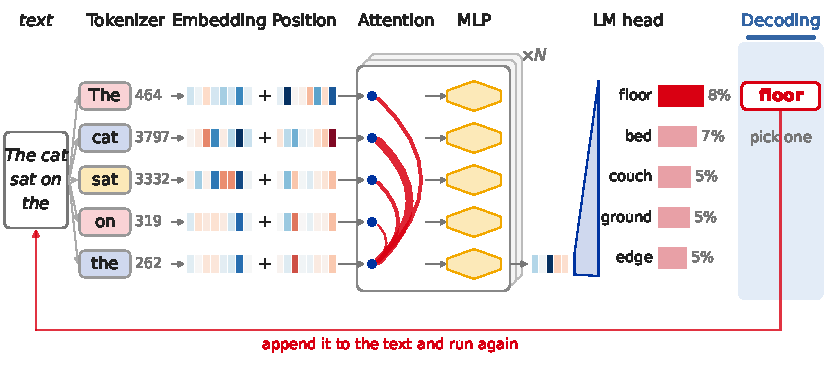
\includegraphics[width=\linewidth]{roadmap_decoding_pass.pdf}\end{center}
  \vskip -2pt
  {\small Today: the last box. The model gives a probability for every token - which one do we
  write?}
\end{frame}

\begin{frame}{Where we are: the life of a model}
  \begin{center}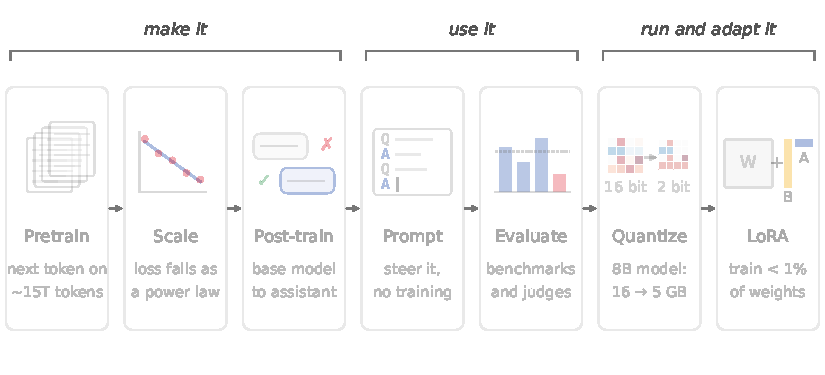
\includegraphics[width=\linewidth]{roadmap_decoding_life.pdf}\end{center}
  \vskip -2pt
  {\small Later: where those probabilities come from, and what you do with a model once you have
  one.}
\end{frame}

% ============================================================ COLD OPEN
\begin{frame}{Always write the best word}
  \vskip 30pt
  \begin{center}
    {\Large\color{popblue}\textbf{The model always writes its single most likely next token.\\[4pt]
    What does the text look like?}}
    \vskip 18pt
    {\small Prompt: ``The cat sat on the'' - the map's sentence. GPT-2, 50 new tokens.}
    \vskip 24pt
    {\small\color{gray}Commit to an answer.}
  \end{center}
\end{frame}

\begin{frame}{It loops}
  \begin{center}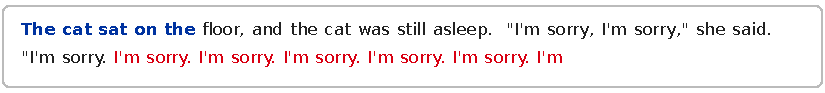
\includegraphics[width=\linewidth]{dec_greedy_loop.pdf}\end{center}
  \vskip -2pt
  {\small GPT-2's real output, always taking the top token (blue: the prompt, red: from the first
  repeat on). It starts well - ``floor'' is the map's 7.6\% favourite - and then it is stuck.}
  \vskip 8pt
  \keybox{So why not just take the top token? That question is today's lecture.}
\end{frame}

\begin{frame}{Outline}
  \tableofcontents
\end{frame}

% ============================================================ 1. WHAT THE MODEL HANDS YOU
\section{What the model hands you}
\sectiontransition{What the model hands you}{A probability for every token. Writing means
choosing one.}

\begin{frame}{One step, one distribution}
  \begin{columns}[T]
    \begin{column}{0.42\textwidth}
      \small
      \begin{itemize}
        \item L21: generate one token, feed it back, repeat.
        \item L26: each step ends in logits $\to$ softmax $\to$ a probability for every one of
          50,257 tokens.
        \item On the map's sentence the favourite, ``floor'', has \textbf{7.6\%}. The top five
          together: 29.6\%. The rest: \textbf{70.4\%}.
      \end{itemize}
    \end{column}
    \begin{column}{0.56\textwidth}
      \vskip -4pt
      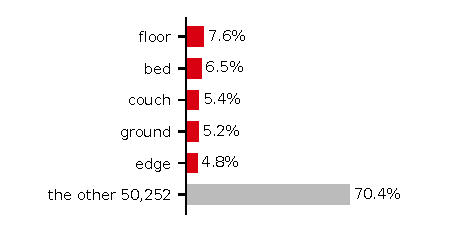
\includegraphics[width=\linewidth]{dec_map_top5.pdf}
    \end{column}
  \end{columns}
  \vskip 8pt
  \keybox{The model never chooses a word. It hands over a distribution; \textbf{decoding} is the
  rule that turns it into one token. Real numbers here: GPT-2 on the map's sentence.}
\end{frame}

\begin{frame}{When to stop}
  \begin{itemize}
    \item \textbf{An end token.} The model writes \texttt{<|endoftext|>} (LLM-1's special token).
      Chat models have an end-of-turn token instead (LLM-6).
    \item \textbf{A length limit.} Stop after $N$ new tokens, whatever happens.
    \item \textbf{Stop strings.} Stop when the text contains, say, ``\textbackslash n\textbackslash
      nUser:''.
  \end{itemize}
  \vskip 8pt
  \watchbox{A stop string can be split across two tokens (LLM-1: tokens are not words). So it is
  checked on the decoded \textbf{text}, not on token IDs.}
\end{frame}

% ============================================================ 2. TAKE THE MOST LIKELY
\section{Take the most likely}
\sectiontransition{Take the most likely}{Greedy, then a smarter greedy.}

\begin{frame}{Greedy}
  \begin{itemize}
    \item At every step write the token with the highest probability (the argmax).
    \item Same input, same output - on one machine (the last section complicates even that).
    \item Why it loops: once a sentence has appeared, writing it again becomes more likely, and
      every repeat makes the next one likelier still. Xu et al. (2022) measured this
      \textbf{self-reinforcement}: the more times a sentence is already in the context, the
      higher its probability of coming next.
  \end{itemize}
  \vskip 8pt
  \keybox{Greedy picks the best \textbf{next} token, one step at a time. It never asks whether
  the whole text is likely.}
\end{frame}

\begin{frame}{Why we work with log-probabilities}
  \small
  The probability of a whole text is the product of its token probabilities. Toy: 100 tokens,
  each with probability 0.1:
  \[
    0.1 \times 0.1 \times \cdots \times 0.1 \;=\; 0.1^{100} \;=\; 10^{-100}
  \]
  \begin{itemize}
    \item The smallest positive number a float32 can hold is about $10^{-45}$. In float32 this
      product is exactly \textbf{0}, and every text scores the same.
    \item Take logs and the product becomes a sum: $100 \cdot \log 0.1 = -230.3$. No underflow,
      and adding is cheaper than multiplying.
    \item Higher (less negative) log-probability = more likely. APIs report \texttt{logprobs}
      per token: a rough confidence signal (calibration, [14]), used to flag shaky answers, to
      rank several candidate answers, and to look for likely hallucinations (LLM-8).
  \end{itemize}
\end{frame}

\begin{frame}{Greedy is short-sighted}
  \begin{center}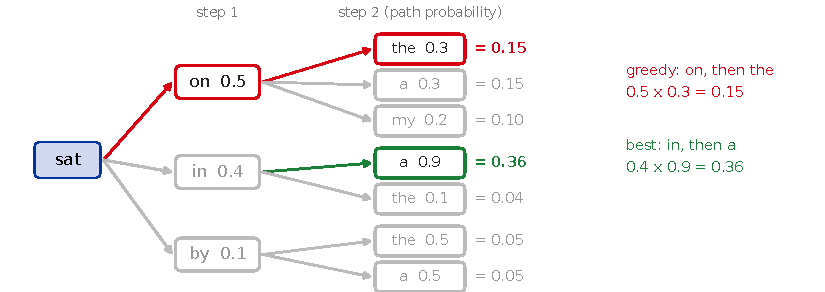
\includegraphics[width=\linewidth]{dec_greedy_tree.pdf}\end{center}
  \vskip -4pt
  {\small Toy numbers. Greedy takes ``on'' (0.5 beats 0.4) and ends with a path of probability
  $0.5 \times 0.3 = 0.15$. The path through ``in'' was $0.4 \times 0.9 = 0.36$, more than twice
  as likely - but greedy never looked one step further.}
\end{frame}

\begin{frame}{By hand: beam search with $B = 2$}
  \begin{center}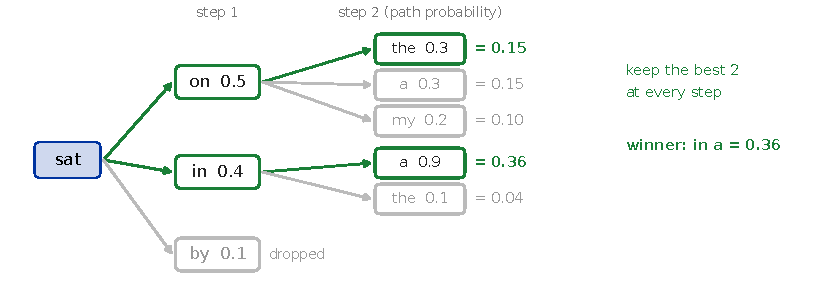
\includegraphics[width=\linewidth]{dec_beam_tree.pdf}\end{center}
  \vskip -4pt
  \small
  Keep the $B$ best \textbf{partial texts} at every step, scored by their total log-probability.
  Step 1 keeps ``on'' and ``in'' and drops ``by''. Step 2 extends both and keeps the two best
  paths: ``in a'' (0.36) and ``on the'' (0.15, tied with ``on a''). The winner is ``in a''.
  With a real vocabulary, each step scores $B \times 50{,}257$ extensions and keeps $B$.
\end{frame}

\begin{frame}{Beam search: why divide by the length}
  \begin{itemize}
    \item Every extra token multiplies the probability by a number below 1, so a longer text
      always has a lower total. Toy: a 3-token ending with 0.5 per token scores
      $0.5^3 = 0.125$; a 6-token ending with 0.7 per token, each step more convincing, scores
      $0.7^6 = 0.118$ and loses.
    \item Plain beam search therefore likes to stop early.
    \item The usual fix: divide the total log-probability by the length (or by the length raised
      to a power, one more knob). Now the 6-token ending wins: average log-probability
      $\log 0.7 = -0.36$ per token against $\log 0.5 = -0.69$.
  \end{itemize}
\end{frame}

\begin{frame}{Predict first}
  \vskip 30pt
  \begin{center}
    {\Large\color{popblue}\textbf{Beam search finds more probable text than greedy.\\[4pt]
    Is more probable text better text?}}
    \vskip 24pt
    {\small\color{gray}Commit to an answer.}
  \end{center}
\end{frame}

\begin{frame}{The probability trap}
  \begin{center}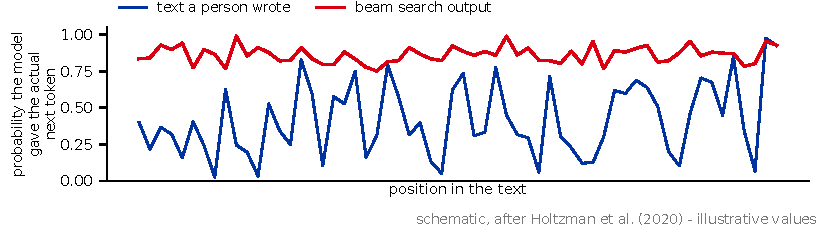
\includegraphics[width=\linewidth]{dec_prob_trap.pdf}\end{center}
  \vskip -4pt
  \small
  At every position of a text, ask: what probability did the model give the token that actually
  came next? Holtzman et al. (2020): for text a person wrote it jumps around and is often low;
  for beam output it stays uniformly high - and that text reads bland and repetitive.
  \vskip 4pt
  \takebox{People write \textbf{surprising} text, not the most probable text. Maximising
  probability is the wrong goal for open-ended writing.}
\end{frame}

\begin{frame}{Where maximising still wins}
  \begin{itemize}
    \item Tasks with \textbf{one right answer} and short outputs: translating a sentence,
      transcribing speech, answering ``what is 17 $\times$ 23?''. Here the most probable output
      is usually the correct one, and translation systems have long used beam search.
    \item Open-ended text - chat, stories, explanations - is the opposite case: many good
      answers, and the single most probable one is dull. Chat models sample.
  \end{itemize}
  \vskip 10pt
  \keybox{Greedy and beam search answer ``what is the most likely text?''. The next section
  answers a different question: ``what would a good writer plausibly write?''.}
\end{frame}

% ============================================================ 3. SAMPLE
\section{Sample}
\sectiontransition{Sample}{Roll the dice - but with which distribution?}

\begin{frame}{Pure sampling and the long tail}
  \begin{center}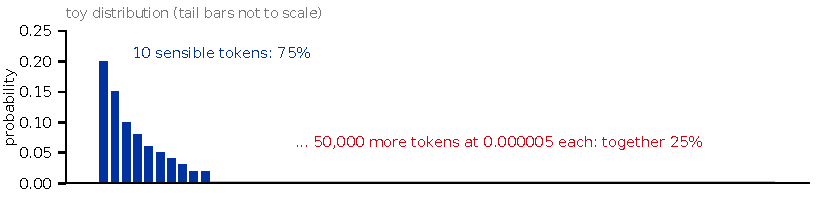
\includegraphics[width=\linewidth]{dec_long_tail.pdf}\end{center}
  \vskip -4pt
  \small
  Sampling straight from the model's distribution fixes the loops: the next token is drawn at
  random, in proportion to its probability. But tens of thousands of unlikely tokens add up. In
  this toy, 50,000 of them at 0.000005 each make \textbf{25\%}: one step in four picks something
  odd, and one odd token can derail every token after it.
  \vskip 4pt
  \keybox{Every sampling method below is a way to reshape the distribution, or cut off its tail,
  before the dice roll.}
\end{frame}

\begin{frame}{Temperature}
  \small
  Divide the logits by a number $T$ before the softmax:
  \[
    p_i \;=\; \frac{e^{z_i / T}}{\sum_j e^{z_j / T}}
  \]
  \begin{itemize}
    \item The same operation as \textbf{temperature scaling} in calibration ([14], and ch11's
      lecture 45): there it fixes over-confidence, here it steers how adventurous the text is.
    \item $T < 1$ widens the gaps between logits: the favourite gets even more probability.
    \item $T > 1$ shrinks the gaps: the distribution flattens.
    \item $T \to 0$: all probability on the top token. That is greedy.
  \end{itemize}
\end{frame}

\begin{frame}{By hand: temperature}
  \small
  Three tokens with logits $z = (2,\ 1,\ 0)$:
  \vskip 6pt
  \textbf{\color{popblue}$T = 1$:}\quad
  $\dfrac{(e^{2},\, e^{1},\, e^{0})}{e^{2} + e^{1} + e^{0}} = \dfrac{(7.39,\ 2.72,\ 1.00)}{11.11}
  = (\mathbf{0.67},\ 0.24,\ 0.09)$
  \vskip 8pt
  \textbf{\color{orange1}$T = 10$:}\quad
  $\dfrac{(e^{0.2},\, e^{0.1},\, e^{0})}{e^{0.2} + e^{0.1} + e^{0}} = \dfrac{(1.22,\ 1.11,\
  1.00)}{3.33} = (0.37,\ 0.33,\ 0.30)$ - nearly uniform
  \vskip 8pt
  \textbf{\color{sampred}$T \to 0$:}\quad the gaps $z_i / T$ grow without bound, so $p \to
  (1,\ 0,\ 0)$: greedy
  \vskip 10pt
  \keybox{Temperature never changes the \textbf{order} of the tokens, only how far apart their
  probabilities are.}
\end{frame}

\begin{frame}{Temperature on the map's sentence}
  \begin{center}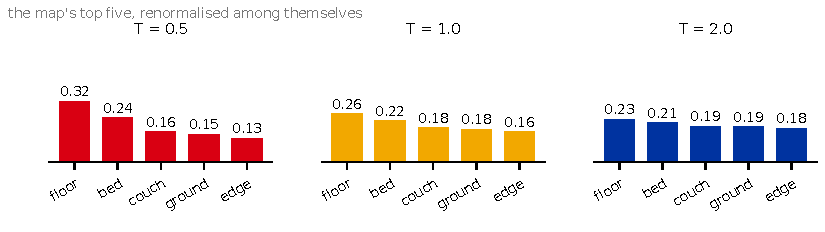
\includegraphics[width=\linewidth]{dec_temperature.pdf}\end{center}
  \vskip -4pt
  {\small The map's real top five, renormalised among themselves at three temperatures. At
  $T = 0.5$ ``floor'' pulls ahead; at $T = 2$ the five are almost level. On the full distribution
  the same happens to all 50,257 tokens: a high temperature hands the long tail more
  probability.}
\end{frame}

\begin{frame}{By hand: temperature and the tail}
  \small
  Dividing the logits by $T$ is the same as raising each probability to the power $1/T$ and
  renormalising. Back to the long-tail toy: 10 sensible tokens with 75\%, 50,000 odd ones at
  0.000005 each (25\%).
  \begin{itemize}
    \item $T = 0.5$: square every probability. The odd tokens' squares are tiny; their share
      falls from 25\% to about \textbf{0.001\%}.
    \item $T = 2$: take square roots. One odd token: $\sqrt{0.000005} = 0.0022$; times 50,000 =
      112. The ten sensible tokens: 2.56 in total. After renormalising, the odd tokens get
      $112 / (112 + 2.56) =$ \textbf{98\%}.
  \end{itemize}
  \vskip 6pt
  \keybox{A high temperature hands the dice to the long tail. That is why temperature is almost
  always combined with a cut-off - the next three slides - and why the order of the two
  matters.}
\end{frame}

\begin{frame}{Top-k, and why a fixed k fails}
  \begin{center}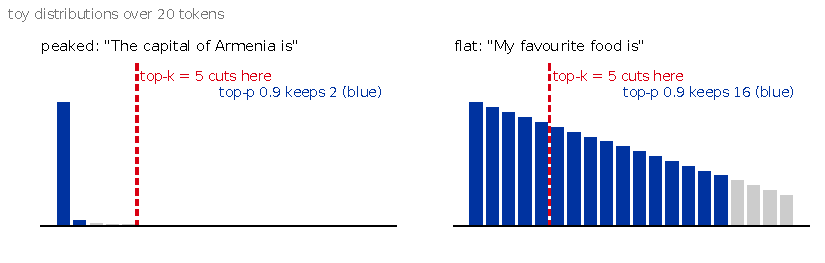
\includegraphics[width=\linewidth]{dec_topk_vs_topp.pdf}\end{center}
  \vskip -4pt
  \small
  \textbf{Top-k}: keep the $k$ most likely tokens, set the rest to 0, renormalise, sample. Toy
  distributions:
  \begin{itemize}
    \item Peaked: one token has 0.88. Keeping 5 lets four unlikely tokens back in.
    \item Flat: 20 tokens from 0.08 down to 0.02. Keeping 5 throws away most of the good ones.
  \end{itemize}
  The right number of candidates changes at every step. A fixed $k$ cannot follow it.
\end{frame}

\begin{frame}{Top-p (nucleus sampling)}
  \begin{itemize}
    \item Top-k's problem was a fixed \textbf{count}. Top-p fixes the \textbf{amount of
      probability} instead: keep the smallest set of top tokens whose probabilities add up to at
      least $p$; renormalise; sample (Holtzman et al., 2020, the same paper as the probability
      trap).
    \item It adapts by itself. Same toys, $p = 0.9$: the peaked one keeps \textbf{2} tokens
      ($0.88 + 0.04 = 0.92$), the flat one keeps \textbf{16}.
    \item The tail of near-zero tokens is cut every time, whatever its size.
  \end{itemize}
  \vskip 10pt
  \keybox{Top-k asks ``how many?''. Top-p asks ``how much probability?'' - and that is the
  question that stays sensible from one step to the next.}
\end{frame}

\begin{frame}{By hand: top-p on the map's sentence}
  \small
  Real numbers, GPT-2 after ``The cat sat on the''. Top-p with $p = 0.2$: add the sorted
  probabilities until the total reaches 0.2.
  \vskip 6pt
  \begin{center}
  \begin{tabular}{lcc}
    \textbf{token} & \textbf{probability} & \textbf{running total} \\
    \hline
    floor  & 0.076 & 0.076 \\
    bed    & 0.065 & 0.141 \\
    couch  & 0.054 & 0.195 \\
    ground & 0.052 & \textbf{0.247} $\geq 0.2$: stop \\
  \end{tabular}
  \end{center}
  \vskip 6pt
  Keep 4 tokens. Renormalise: floor $0.076 / 0.247 = 0.31$, bed $0.26$, couch $0.22$,
  ground $0.21$. Then sample. (A realistic $p$ is 0.9 or more; 0.2 keeps the table short.)
\end{frame}

\begin{frame}{Min-p}
  \small
  \textbf{Min-p}: keep the tokens whose probability is at least min\_p times the top token's.
  Toys, min\_p $= 0.1$:
  \begin{itemize}
    \item Peaked: the top is 0.88, so the bar is 0.088 - only \textbf{1} token passes.
    \item Flat: the top is 0.08, so the bar is 0.008 - all \textbf{20} pass.
  \end{itemize}
  Like top-p it adapts, through a cut-off that scales with the model's confidence.
  \vskip 6pt
  \keybox{The gap it targets, its authors argue: at a high temperature the distribution flattens
  (the tail slide), and top-p's set fills with weak tokens. Min-p's bar is tied to the top
  token, so it stays strict whenever the model has a clear favourite.}
\end{frame}

\begin{frame}{How to read a claim: min-p}
  \begin{itemize}
    \item Min-p was an oral presentation at ICLR 2025 (Nguyen et al.), one of the
      highest-scored papers, with claims of better quality and diversity than top-p.
    \item A 2025 re-analysis (``Min-p, Max Exaggeration'', arXiv 2506.13681) found that it does
      not beat the standard samplers once they are tuned with the same effort, and found
      inconsistencies in how the original results were reported.
    \item Min-p is still a reasonable sampler - llama.cpp turns it on by default. What fell was
      the claim that it is better.
  \end{itemize}
  \vskip 10pt
  \watchbox{An oral at a top venue is a starting point, not the last word. Ask: compared with
  what, tuned how hard, and measured by whom?}
\end{frame}

\begin{frame}{The order of the knobs}
  \begin{center}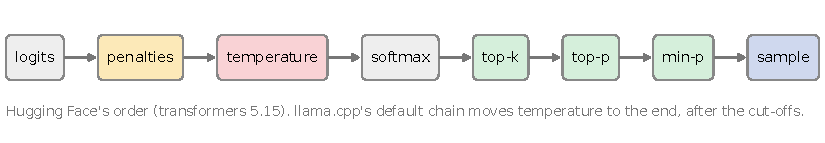
\includegraphics[width=\linewidth]{dec_knob_pipeline.pdf}\end{center}
  \vskip 2pt
  \small
  \begin{itemize}
    \item Greedy is the special case $T \to 0$, or top-k with $k = 1$.
    \item Libraries do not agree on the order. Hugging Face applies temperature \textbf{before}
      the cut-offs; llama.cpp's default chain applies it \textbf{last}. With top-p or min-p that
      changes which tokens survive: a high temperature flattens the distribution first, and
      top-p then keeps more tokens.
  \end{itemize}
  \vskip 4pt
  \watchbox{``temperature 0.8, top-p 0.95'' is not one setting. Check the library.}
  \vskip 2pt
  \src{transformers 5.15 \texttt{generate()} source; llama.cpp \texttt{--samplers} default:
  penalties; ...; top\_k; ...; top\_p; min\_p; ...; temperature. Checked 5 Oct 2026.}
\end{frame}

\begin{frame}{By hand: the order matters}
  \small
  Toy distribution $(0.5,\ 0.3,\ 0.15,\ 0.05)$, temperature $T = 2$, top-p $= 0.8$:
  \vskip 6pt
  \textbf{Temperature first} (Hugging Face): square roots, renormalised:
  $(0.38,\ 0.29,\ 0.21,\ 0.12)$. Top-p 0.8: $0.38 + 0.29 = 0.67$, plus $0.21 = 0.88$ - keep
  \textbf{3} tokens.
  \vskip 6pt
  \textbf{Cut first} (llama.cpp's default chain): top-p 0.8 on the original: $0.5 + 0.3 = 0.80$ -
  keep \textbf{2} tokens. Temperature then flattens just those two.
  \vskip 10pt
  \takebox{Same two settings, different sets of candidates. The third token can only ever be
  written in the first library.}
\end{frame}

\begin{frame}{Repetition penalties: two different things}
  \small
  \begin{itemize}
    \item \textbf{Multiplicative} (Keskar et al., 2019, the CTRL paper; Hugging Face's and
      llama.cpp's \texttt{repetition\_penalty}): for every token already in the text, divide its
      logit by the penalty (multiply it, if the logit is negative). Toy, penalty 1.3: a logit of
      2.6 becomes 2.0.
    \item \textbf{Subtractive} (OpenAI's API): subtract a fixed amount from every token that has
      appeared (presence penalty), plus an amount per appearance (frequency penalty):
      \[
        z_j \;\leftarrow\; z_j - c_j \cdot \alpha_{\text{frequency}} - [c_j > 0] \cdot
        \alpha_{\text{presence}}
      \]
      where $c_j$ counts how often token $j$ has appeared. Toy: a token used 3 times, both
      penalties 0.5: its logit drops by $1.5 + 0.5 = 2.0$.
  \end{itemize}
  \vskip 4pt
  \watchbox{Same name, different maths, different scales. Too strong and the model avoids
  words it genuinely needs to repeat - names, ``the''.}
\end{frame}

\begin{frame}{Seeds}
  \begin{itemize}
    \item Sampling draws random numbers, so the same prompt gives different texts on different
      runs. That is the point of sampling.
    \item A fixed \textbf{seed} replays the same random numbers, so the same text comes out
      again - on the same machine, with the same software and the same settings.
    \item Useful for debugging and for comparing two prompts fairly.
  \end{itemize}
  \vskip 10pt
  \keybox{``On the same machine'' is doing a lot of work in that sentence. The last section shows
  why.}
\end{frame}

\begin{frame}{Settings in practice}
  \small
  \begin{itemize}
    \item One real set of defaults: llama.cpp ships temperature 0.8, top-k 40, top-p 0.95,
      min-p 0.05 (\texttt{llama-cli} documentation, checked 5 Oct 2026). All four filters are on
      at once.
    \item Lower temperature for code, maths and facts, where one answer is right; higher for
      brainstorming and fiction, where variety is the point.
    \item Change one knob at a time, and read your library's documentation for the order.
  \end{itemize}
  \vskip 10pt
  \keybox{These are habits, not laws. The right setting depends on the model and on the task.}
\end{frame}

\begin{frame}{What you see, what to change}
  \footnotesize
  \begin{center}
  \begin{tabular}{>{\raggedright\arraybackslash}p{3.4cm}>{\raggedright\arraybackslash}p{4.0cm}%
                  >{\raggedright\arraybackslash}p{4.4cm}}
    \textbf{what you see} & \textbf{likely cause} & \textbf{try} \\
    \hline
    the text loops & greedy, or a very low temperature & sample; raise the temperature a little;
      a mild repetition penalty \\[3pt]
    odd words, sudden nonsense & the long tail: temperature too high, or no cut-off & lower the
      temperature; add top-p (or top-k, min-p) \\[3pt]
    bland, the same answer every time & too little randomness & raise the temperature \\[3pt]
    needed words avoided (names, ``the'') & repetition penalty too strong & lower it \\[3pt]
    broken JSON & free sampling & constrain the choice (next section) \\[3pt]
    different answers at temperature 0 & the server's arithmetic (real-systems section) & accept it, or
      batch-invariant serving \\
  \end{tabular}
  \end{center}
  \vskip 6pt
  \keybox{One knob at a time, one symptom at a time.}
\end{frame}

% ============================================================ 4. CONSTRAIN THE CHOICE
\section{Constrain the choice}
\sectiontransition{Constrain the choice}{When the output must follow a format. Not a third
option: a filter on top of either.}

\begin{frame}{Masking}
  \begin{itemize}
    \item At every step, find every token that would make the output break the required format
      - a schema for JSON (JavaScript Object Notation, the text format programs exchange data
      in), a list of allowed answers, any grammar.
    \item Set their logits to $-\infty$, so their probability is 0. Renormalise the rest.
    \item Then pick as usual: greedy, beam, or sampled with any of the knobs above.
  \end{itemize}
  \vskip 10pt
  \keybox{The model is not retrained and does not ``know'' about the format. The decoder simply
  never lets it write an illegal token.}
\end{frame}

\begin{frame}{By hand: JSON}
  \begin{center}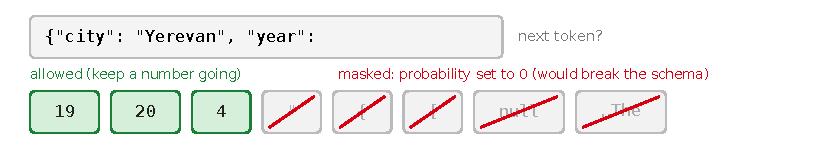
\includegraphics[width=\linewidth]{dec_json_mask.pdf}\end{center}
  \vskip -2pt
  \small
  The schema says \texttt{\{"city": string, "year": integer\}}, and the output so far ends
  with \texttt{"year":} - so a number must come next. Only tokens that continue a number are
  legal; a quote,
  a brace, \texttt{null} or a word are masked, however much probability the model gave them.
  The mask covers all 50,000+ tokens at every step, not just the eight drawn.
\end{frame}

\begin{frame}{Tokens are not characters}
  \begin{itemize}
    \item LLM-1: one token can hold several characters, like \texttt{":} or \texttt{"\}}, which
      cover two steps of the grammar at once.
    \item So the mask cannot look at one character at a time. For every token it checks the
      token's whole text against the grammar from the current state.
    \item Doing that for 50,000 tokens at every step would be slow, so libraries precompute,
      for each state of the grammar, which tokens are legal.
  \end{itemize}
\end{frame}

\begin{frame}{What it buys, and what it does not}
  \begin{itemize}
    \item \textbf{Guaranteed format.} Tool calls for agents (L44) and JSON for programs to read
      always parse.
    \item \textbf{Not guaranteed truth.} A valid \texttt{"year"} can still be the wrong year.
    \item \textbf{Not guaranteed complete.} Hit the length limit in the middle of an object and
      the JSON is cut off anyway.
  \end{itemize}
  \vskip 10pt
  \watchbox{Constrained decoding checks the shape of the answer, never its content.}
\end{frame}

% ============================================================ 5. REAL SYSTEMS
\section{Real systems}
\sectiontransition{Real systems}{What changes when a server does the decoding.}

\begin{frame}{Streaming: stopping in the middle of a letter}
  \begin{center}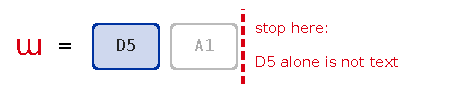
\includegraphics[width=3.0in]{dec_ayb_bytes.pdf}\end{center}
  \vskip 2pt
  \begin{itemize}
    \item Chat apps show tokens as they arrive (streaming), not after the whole answer is done.
    \item LLM-1: in UTF-8 the Armenian letter ayb is two bytes, D5 A1, and a byte-level
      tokenizer can give each byte its own token.
    \item A token holding only D5 is not text yet. Show it - or hit the length limit right after
      it - and the screen gets a broken character. So the app must hold back bytes until a
      character is complete.
  \end{itemize}
\end{frame}

\begin{frame}{Predict first}
  \vskip 30pt
  \begin{center}
    {\Large\color{popblue}\textbf{Temperature 0. The same prompt, 1,000 times.\\[4pt]
    How many different answers?}}
    \vskip 24pt
    {\small\color{gray}Commit to an answer.}
  \end{center}
\end{frame}

\begin{frame}{Temperature 0 is not deterministic}
  \small
  Thinking Machines Lab (He, Sept 2025): Qwen3-235B-A22B-Instruct, 1,000 runs, temperature 0 -
  \textbf{80 different completions}. The most common one appeared 78 times.
  \vskip 6pt
  \begin{itemize}
    \item Floating-point addition depends on the order. Toy, in float32:
      $(10^8 + 1) - 10^8 = 0$, but $(10^8 - 10^8) + 1 = 1$.
    \item A server runs many users' requests together as one big matrix multiplication: a
      \textbf{batch}. The GPU program for each operation (a \textbf{kernel}) splits long sums into
      chunks, and how it splits depends on the batch size - which changes with the load, second
      to second.
    \item So your logits differ in the last digits from run to run. Usually nothing changes; when
      two tokens are nearly tied, the argmax flips and every later token follows a new path.
      Flips land at different places in different runs: 80 different texts.
  \end{itemize}
  \vskip 4pt
  \takebox{Their fix, batch-invariant kernels, makes all 1,000 identical, at a cost in speed.
  Greedy decoding is deterministic; the arithmetic underneath it may not be.}
\end{frame}

\begin{frame}{Why decoding is slow}
  \begin{itemize}
    \item One token per step, and every step is a full forward pass through every layer. 500
      tokens of answer = 500 passes, one after another.
    \item For a single token the GPU has little arithmetic to do, but it must read all of the
      model's weights from memory each time. Decoding is limited by memory, not by arithmetic
      (the details are LLM-11).
    \item Checking several tokens in one pass costs about as much as checking one.
  \end{itemize}
  \vskip 10pt
  \keybox{That last point is the whole trick of the next slide.}
\end{frame}

\begin{frame}{Speculative decoding}
  \begin{center}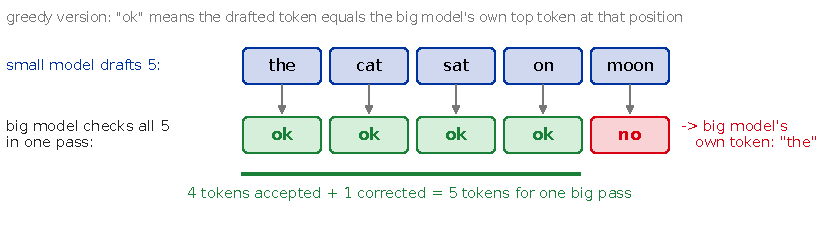
\includegraphics[width=\linewidth]{dec_speculative.pdf}\end{center}
  \vskip -4pt
  \small
  \begin{itemize}
    \item A small, fast model \textbf{drafts} $k$ tokens, one at a time.
    \item The big model checks all $k$ in \textbf{one} pass: the causal mask (L25) gives its
      prediction at every position at once.
    \item Keep the drafted tokens up to the first disagreement, take the big model's own token
      there, and draft again.
  \end{itemize}
  \src{Leviathan, Kalman \& Matias (2023), ICML; Chen et al. (2023), DeepMind.}
\end{frame}

\begin{frame}{By hand: accept or reject}
  \small
  \textbf{Greedy}: accept a drafted token if it equals the big model's own top token. The
  output is then exactly what the big model would have written alone.
  \vskip 6pt
  \textbf{Sampling}: accept a drafted token $x$ with probability
  $\min\!\big(1,\; p_{\text{big}}(x) / p_{\text{small}}(x)\big)$. Toy: the small model gave $x$
  0.6, the big one 0.3: accept half the time. On a reject, sample from what the big model wanted
  \textbf{more} than the small one did.
  \vskip 8pt
  \keybox{Both halves together give tokens with exactly the big model's probabilities - next
  slide, by hand. \textbf{Lossless}: no quality traded for speed. Leviathan et al. report
  2-3$\times$ faster generation with T5-XXL.}
  \vskip 4pt
  {\small When the draft is good, most tokens are accepted and each big pass yields several
  tokens; when it is bad, it costs little more than plain decoding.}
\end{frame}

\begin{frame}{By hand: why sampling stays lossless}
  \small
  Three tokens. Small model $p_s = (0.6,\ 0.3,\ 0.1)$, big model $p_b = (0.3,\ 0.5,\ 0.2)$. The
  small model drafts a token; we accept it with probability $\min(1, p_b / p_s)$.
  \vskip 4pt
  \begin{center}
  \begin{tabular}{lccccc}
    \textbf{token} & \textbf{drafted} $p_s$ & \textbf{accept} & \textbf{kept} &
      \textbf{shortfall} $\max(0, p_b - p_s)$ & \textbf{total} \\
    \hline
    A & 0.6 & 0.5 & 0.30 & 0   & $0.30 + 0 = $ \textbf{0.30} \\
    B & 0.3 & 1   & 0.30 & 0.2 & $0.30 + 0.20 = $ \textbf{0.50} \\
    C & 0.1 & 1   & 0.10 & 0.1 & $0.10 + 0.10 = $ \textbf{0.20} \\
  \end{tabular}
  \end{center}
  \vskip 4pt
  \begin{itemize}
    \item Kept: $0.30 + 0.30 + 0.10 = 0.70$, so a reject happens with probability 0.30 (only A
      is ever rejected: the small model was over-eager about it).
    \item On a reject, sample from the shortfall $(0,\ 0.2,\ 0.1)$, renormalised:
      $(0,\ \tfrac{2}{3},\ \tfrac{1}{3})$. That adds $0.30 \times (0,\ \tfrac{2}{3},\
      \tfrac{1}{3}) = (0,\ 0.20,\ 0.10)$.
  \end{itemize}
  \takebox{Totals $(0.30,\ 0.50,\ 0.20)$: exactly the big model. Keep what the small model did
  not overdo, resample exactly what it underdid. (The name for this trick: rejection sampling.)}
\end{frame}

\begin{frame}{Where the draft comes from}
  \begin{itemize}
    \item A small model of the same family, with the same tokenizer.
    \item Extra prediction heads trained on top of the big model itself.
    \item Copying: in summaries and code edits the next tokens are often already in the prompt.
    \item Multi-token prediction: models trained to guess several tokens at once (LLM-11).
  \end{itemize}
  \vskip 10pt
  \takebox{Speculative decoding changes \textbf{how fast} tokens come out, never \textbf{which}
  tokens come out. That is why serving systems can switch it on silently.}
\end{frame}

\begin{frame}{Watermarking lives in the sampler}
  \small
  SynthID-Text (Dathathri et al., \emph{Nature}, 2024), used in Google's Gemini:
  \begin{itemize}
    \item When several candidate tokens are about equally good, a secret, keyed function
      decides which one wins. The model itself is untouched; only the sampling step changes.
    \item Anyone with the key can score a text: if its token choices agree with the keyed
      function far more often than chance, it is watermarked. Toy: the function prefers half of
      all candidates, so ordinary text hits a preferred token about 50\% of the time;
      watermarked text, say, 70\%. Over a few hundred tokens that gap cannot be luck.
    \item A reader cannot see anything: every token was a plausible choice anyway.
  \end{itemize}
  \vskip 4pt
  \watchbox{Google's own documentation: weaker on factual answers (with one right answer there is
  no freedom to hide a signal) and when a text is thoroughly rewritten or translated.}
\end{frame}

% ============================================================ RECAP
\section*{Recap}

\begin{frame}{Recap}
  \begin{itemize}
    \item The model hands over a probability for every token; \textbf{decoding} picks one. Stop
      on an end token, a length limit or a stop string.
    \item \textbf{Take the most likely}: greedy (loops, short-sighted), beam search (looks ahead;
      right for one-right-answer tasks, bland for open-ended text).
    \item \textbf{Sample}: temperature reshapes; top-k, top-p and min-p cut the tail; penalties
      discourage loops. Libraries differ in the order.
    \item \textbf{Constrain}: masks guarantee a format, not the truth.
    \item \textbf{Real systems}: temperature 0 can still drift; speculative decoding is free
      speed; a watermark can hide in the sampler.
  \end{itemize}
\end{frame}

\begin{frame}{Next on the map}
  \begin{center}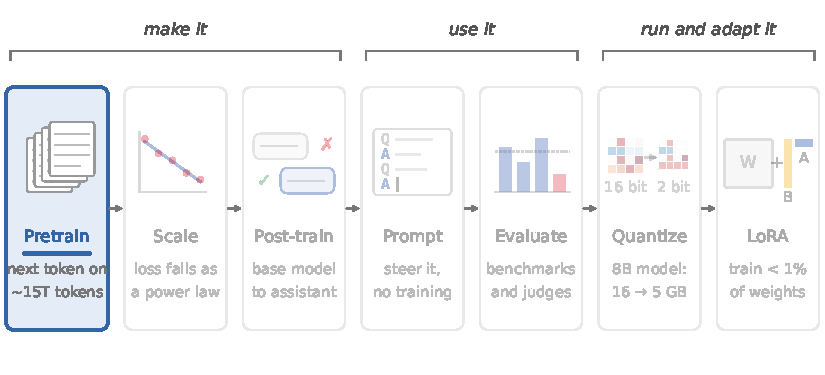
\includegraphics[width=\linewidth]{roadmap_pretraining_life.pdf}\end{center}
  \vskip -2pt
  {\small Next (LLM-4): where these probabilities come from - pretraining.}
\end{frame}

\begin{frame}{Sources \& further reading}
  \footnotesize
  \begin{itemize}
    \item Holtzman, Buys, Du, Forbes \& Choi (2020), ``The Curious Case of Neural Text
      Degeneration'', ICLR (the probability trap, top-p).
    \item Xu et al. (2022), ``Learning to Break the Loop'', NeurIPS (self-reinforcing repetition).
    \item Keskar et al. (2019), ``CTRL'' (the repetition penalty); OpenAI API documentation
      (presence and frequency penalties).
    \item Nguyen et al. (2025), ``Turning Up the Heat: Min-p Sampling'', ICLR; ``Min-p, Max
      Exaggeration'' (2025), arXiv 2506.13681.
    \item He / Thinking Machines Lab (10 Sept 2025), ``Defeating Nondeterminism in LLM
      Inference''.
    \item Leviathan, Kalman \& Matias (2023), ``Fast Inference from Transformers via Speculative
      Decoding'', ICML; Chen et al. (2023), ``Accelerating Large Language Model Decoding with
      Speculative Sampling''.
    \item Dathathri et al. (2024), ``Scalable watermarking for identifying large language model
      outputs'', \emph{Nature}.
  \end{itemize}
  \vskip 2pt
  \src{Figures: \texttt{py\_src/decoding\_figs.py} (toy numbers; GPT-2's greedy output and the
  map's top five are the only real ones).}
\end{frame}

\end{document}

% ============================================================================
% Provenance:
%   Deck: LLM-3 Decoding (14_llms), session 6 of the LLM chapter. Built 2026-10-05 from
%   LLM3_decoding_OUTLINE.md (critique + interview 2026-10-05, self-reviewed) and
%   LLM_CHAPTER_PLAN.md, section 5 (LLM-3). Ported and adapted from the instructor's DL4NLP deck
%   4 (sources/dl4nlp/04_decoding_strategies.tex): the temperature worked example (corrected:
%   e^2 / (e^2 + e + 1) = 0.665 rounds to 0.67, the source printed .66), beam search B = 2 (new
%   toy numbers), the knob pipeline, structured decoding and its JSON example, the speculative
%   decoding frames. Cut: contrastive search, the API-parameter table, "Common questions".
%   Interview decisions: cold open "GPT-2 loops"; real systems = temperature 0 not deterministic,
%   speculative decoding (moved here from LLM-11), watermarking (not: providers locking knobs);
%   min-p taught with the 2025 critique; no hands-on in the slides.
%   Numbers (ml/SLIDE_STYLE.md, 2026-10-05): toy by default. Real: GPT-2's greedy continuation of
%   "The cat sat on the" (cached model, decoding_figs.py --gpt2 -> results/decoding_gpt2.json;
%   six prompts tried, all looped) and the map's top five (results/roadmap_gpt2.json).
%   Verified 2026-10-05: llama.cpp --samplers default order (temperature last) and defaults
%   (temp 0.8, top-k 40, top-p 0.95, min-p 0.05) from its README via Context7; Hugging Face order
%   (repetition penalty, temperature, top-k, top-p, min-p) from the installed transformers 5.15
%   generation/utils.py; OpenAI penalty formula; Xu et al. NeurIPS 2022 self-reinforcement;
%   Thinking Machines primary post (Qwen3-235B-A22B-Instruct-2507, 80 unique of 1,000, most common
%   78; cause: batch size varies with load - secondary write-ups said Qwen3-8B, wrongly); min-p
%   ICLR 2025 oral + arXiv 2506.13681; SynthID-Text Nature 2024 + Google's stated limits.
%   SELF-REVIEW 2026-10-05: detectors 0/0/0, acronyms pass (JSON spelled out in "Masking"; the
%   undefined "KV cache" forward reference removed). Caught by the asserts and the clipping check:
%   the top-5 sum is 29.6% (29.5 was a sum of rounded values); the by-hand top-p table adds the
%   printed 3-decimal values (.141/.195/.247; unrounded .142/.196/.248 keep the same 4 tokens).
%   Caught by eye: the speculative figure's correction after "the cat sat on" said "mat" - it is
%   "the" (the source deck had it right); the JSON frame's sentence; one 1 pt overfull column.
%   STUDENT REVIEW 2026-10-05 (one Sonnet agent, rendered PNGs only, pedagogy brief; ~104k
%   tokens, 87 s). Applied (worked examples and missing steps; toys asserted in review_toys):
%   "By hand: why sampling stays lossless" (p_s (0.6,0.3,0.1), p_b (0.3,0.5,0.2): kept
%   (0.30,0.30,0.10), reject 0.30, shortfall (0,2/3,1/3) -> totals = p_b exactly; "rejection
%   sampling" only named, since the course never taught it); the speculative figure labelled as
%   the greedy version; "By hand: temperature and the tail" (long-tail toy: tail share 0.001% at
%   T = 0.5, 25% at 1, 98% at 2); "By hand: the order matters" (T = 2 then top-p 0.8 keeps 3;
%   cut first keeps 2); "Which knob fixes what" replaced by a symptom -> cause -> try table;
%   top-k -> top-p -> min-p signposted as each fixing the previous gap; the min-p critique on its
%   own frame; temperature 0: batch and kernel defined, chunked sums, why flips give 80 texts;
%   the probability-trap plot says what it plots; the half-letter frame moved to Real systems as
%   streaming; logprobs uses; beam's B x vocabulary; a SynthID scoring toy. Not applied: cutting
%   the draft-sources frame, a grammar state table, a mechanism for self-reinforcement beyond
%   Xu et al.'s measurement.
%   Forward pointer: LLM-4 pretraining.
% ============================================================================
